\documentclass[a4paper, 12pt, twocolumn]{article}

\input{bnumath}
\usepackage{makeidx}
\makeindex
\usepackage{color}
\usepackage[all,pdf]{xy}
\usepackage{graphicx}
\usepackage{asymptote}
\usepackage{txfonts}
\usepackage{listings}
\usepackage[left=2cm, right=2cm, top=2cm, bottom=2cm]{geometry}


\title{Cloud Resource Allocation Learning}
\author{
    Tong Cheng\thanks{Done during the internship.} \\
    MSRA 
    \and 
    Hang Dong \\
    MSRA}
\date{Jan 10, 2022}

\begin{document}
\maketitle
\tableofcontents
\section{Introduction}

Arity\index{Arity}: arity of relation $R$ is the number of columns in relation $R$.

free tuple may use either variables or constants.

conjunctive query, query, query mapping

\section{Background}

\begin{equation}
\left(
\begin{array}{ccc|c}
   a_{11} & a_{12} & a_{13} & b_{1} \\
   a_{21} & a_{22} & a_{23} & b_{2} \\
   a_{31} & a_{32} & a_{33} & b_{3} \\
\end{array}
\right)    
\end{equation}

\color{red}Red text collide with \textcolor{blue}{blue} text.

\colorbox{yellow}{Yellow mark}
\color{black}

\section{XY-pic Illustrations}

\xymatrix{
    a & b\ar[rd] & a+b \\
    1 & 2 & 3\ar"1,1"
    \ar"1,1";"2,2"
}

\xymatrix{
    A\ar[r]^{\alpha} & B\ar[d]_{\beta} \\
    C\ar[ur]|{\Sigma} & D
}

\xymatrix{
    A\ar[rd]|\hole & B \\
    C\ar[ru] & D \\
}

\begin{figure}
    \centering
    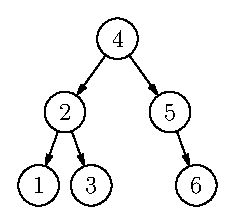
\includegraphics{fig}
    \caption{Binary Tree}
\end{figure}

\begin{asy}
    real r = 0.8cm;
    for (int i = 0; i < 360; i+=10)
        draw(circle(dir(i)*r, r));
\end{asy}

\section{Body}

"It is Kunth's book."

\[
    1 + 2 = 3
    \]

\begin{equation}
    3 + 4 = 7
\end{equation}

$90\degree$

\[
    \int_0^1 f(t) \dif t
    \]

\[
    \frac 12 + \frac 1a = \frac{2+a}{2a}
    \]

$\realf$ is the real field. $\directSum_{i=1}^{n} P_i$ is the direct sum.

\begin{subequations}
    \begin{alignat}{1}
       a_{11} x + a_{12} y + a_{13} z = A \\
       a_{21} x + a_{22} y + a_{23} z = B \\
       a_{31} x + a_{32} y + a_{33} z = C 
    \end{alignat}
\end{subequations}

\begin{equation}
    \begin{split}
        \left| A_1 \union A_2 \union \dots \union A_n \right| = 
            \sum_{1 \leq i_1 \leq n} |A_{i_1}| - \\
            + \sum_{} |A_{i_1} \intersect|\\
    \end{split}
\end{equation}


\section{Code}
\lstset{
    basicstyle=\sffamily,
    keywordstyle=\bfseries,
    commentstyle=\rmfamily\itshape,
    stringstyle=\ttfamily
}
\begin{lstlisting}[language=C]
    #include <stdio.h>
    int main(){
        printf("Hello world.");
    }
\end{lstlisting}


\printindex
\end{document}